\documentclass[12pt, letterpaper]{article}
\date{\today}
\usepackage[margin=1in]{geometry}
\usepackage{amsmath}
\usepackage{hyperref}
\usepackage{cancel}
\usepackage{amssymb}
\usepackage{fancyhdr}
\usepackage{pgfplots}
\usepackage{booktabs}
\usepackage{pifont}
\usepackage{amsthm,latexsym,amsfonts,graphicx,epsfig,comment}
\pgfplotsset{compat=1.16}
\usepackage{xcolor}
\usepackage{tikz}
\usetikzlibrary{shapes.geometric}
\usetikzlibrary{arrows.meta,arrows}
\newcommand{\Z}{\mathbb{Z}}
\newcommand{\N}{\mathbb{N}}
\newcommand{\R}{\mathbb{R}}
\newcommand{\Q}{\mathbb{Q}}
\newcommand{\C}{\mathbb{C}}

\newcommand{\Po}{\mathcal{P}}
\newcommand{\Pro}{\mathbb{P}}
\author{Alex Valentino}
\title{451 homework}
\pagestyle{fancy}
\renewcommand{\headrulewidth}{0pt}
\renewcommand{\footrulewidth}{0pt}
\fancyhf{}
\rhead{
	Homework 9\\
	451	
}
\lhead{
	Alex Valentino\\
}
\begin{document}
\begin{enumerate}
	\item[1.4]
	\begin{enumerate}
		\item Suppose $S \subset R, S$ is a simple module, $S \neq \emptyset$.  Additionally, consider the map $\psi : R \to S$ given by $\psi (r) = rs,$ where
		$s \in S$.  We can say this because $S \neq \emptyset$.  Note that $\psi$
		is surjective because $Im \psi$ is a submodule of $S$, and if $Im \psi \neq S$ then $S$ would have a proper submodule, contradicting the simplicity of S.
		Since $\psi$ is surjective then we can apply the correspondence theorem.
		Since $S$ has no proper submodules, then it contains exactly 2 ideals.  
		This means that $S$ is a field over the ring $R$.  Therefore the kernel 
		of $\psi$ must be maximal.  Therefore by the first isomorphism theorem 
		$S \cong R / \ker \psi $
		\item Suppose $S, S'$ are simple modules and $\phi S \to S'$ is a homomorphism.  Suppose that $\phi$ is not the zero map.  Then for all $s \in S$,
		$\phi(s) \neq 0$.  We know by the previously proved theorem that $S,S'$ are isomorphic to $R/M, R'/M'$, where $M,M'$ are maximal ideals.  
	\end{enumerate}
	\item[2.1] We claim that $M = (x,y)$ is not a free module over $\C[x,y]$.
	First we claim that the size of the basis must be greater than 1.  Assume for 
	contradiction that a single element $g \in (x,y)$ can generate $(x,y)$.  
	Then there must exists $p,q \in \C[x,y]$ such that $pg = x, qg = y$.  
	Since $x,y$ are irreducible, then $g$ must be a unit.  
	However, the only units of $\C[x,y]$ are $\{-1,1,i,-i\}$.  Since every element 
	in $(x,y)$ is a linear combination of the variables $x$ and $y$ then every 
	element in $M$ is a polynomial.  Thus $\{-1,1,i,-i\} \subset \C \not \subset M$.  Thus the basis of $(x,y)$ must contain greater than 1 element.  Suppose 
	$b_1,\cdots,b_n \in M$ is a basis of $M$.  Then if $n$ is even we can have 
	for each $b_i$ to be multiplied by $(-1)^i\prod_{j=1, i\neq j}^n$.  Thus every 
	element is either the negative product of all the basis elements or positive. 
	Thus their sum is 0.  If $n$ is odd we can simply choose to multiply $b_n$ by 0
	then repeat the process for the evens.  Thus $b_1,\cdots,b_n$ is not linearly 
	independent.  Thus $M$ is not a free module since it lacks a basis.  
	\item[2.3] Let $\varphi : \Z^n \to \Z^m$ be given by $\varphi(x) = Ax$
	\begin{enumerate}
		\item 
		\begin{itemize}
			\item $\Rightarrow$ Suppose $\varphi$ is injective.  We want to show that 
			$\varphi$ has a trivial kernel.  Suppose for contradiction that 
			$\ker \phi \neq \{0\}$.  Then there exists 
			$x \in \Z^n, x \neq 0, \phi(x) = 0$.  Therefore we can consider that 
			$x$ and $2x$ under $\phi,$ where $x \neq 2x$ yet 
			$\varphi(x) = 0 = 2*0 = 2* \varphi(x) = \varphi(2x)$.  
			This contradicts the injectivity of $\varphi$.  Thus $\ker \varphi$ 
			is trivial.  Note that this kernel is over $\Z^n$, however this isn't
			an issue. If there was a rational solution to $\varphi(v) = 0$, with 
			$v = (\frac{a_1}{b_1},\cdots, \frac{a_n}{b_n})$, then one can multiply
			both sides of $\varphi(v) = 0$ by $\prod_{i=1}^n b_i$, giving us 
			$\prod_{i=1}^n b_i v \in \Z^n$ and $\varphi(\prod_{i=1}^n b_i v) = 0$.
			Thus a trivial kernel over $\Z$ is equivalent to a trivial kernel over
			$\Q$.  And since our equations are just multiplying and adding integers
			then our solutions will always be rational.  Thus we have a trivial 
			real kernel for our matrix.  
			Thus by rank nullity $n = rank(A) + nullity(A) = rank(A) + 0 = rank(A).$
			\item $\Leftarrow$ Suppose $\varphi$ is not injective.  Then there 
			exists $x,y \in \Z^n$ such that $x \neq y$ and 
			$\varphi(x) = \varphi(y)$.
			Thus $\varphi(x-y) = 0$ and $x-y \neq 0$.  
			Thus $\varphi$ has a non-trivial	kernel.  Thus by rank-nullity 
			$n = rank(A) + nullity(A) \geq rank(A) + 1, n-1 \geq rank(A)$.  
			Therefore $n \neq rank(A)$.  
		\end{itemize}
		\item Note that with the 3 integer row (column) operations (1. row swap, 2. multiplying a row by -1, row addition), the first two simply change the sign, 
		which the gcd is invariant under, and for adding two rows, if the minor 
		contains a portion of both rows then the gcd is unchanged, and if the 
		minor have one of the rows then the gcd has the invariant $gcd(a,b) = gcd(a, b+a)$.  Since row and column operations preserve the gcd of the determinates 
		of the minor, then the matrix should have the same gcd of the determinates
		of minors of the matrix in smith normal form.  Note that the matrix being
		in smith normal form means that exactly one of the m by m minors can be 
		non-zero.  Thus having a determinate of an integer matrix with only a diagonal be 1 is exactly equivalent to the diagonal being 1s.  Having a diagonal be
		all 1s is equivalent to the matrix being surjective.    
	\end{enumerate}
	\item[4.1a]
	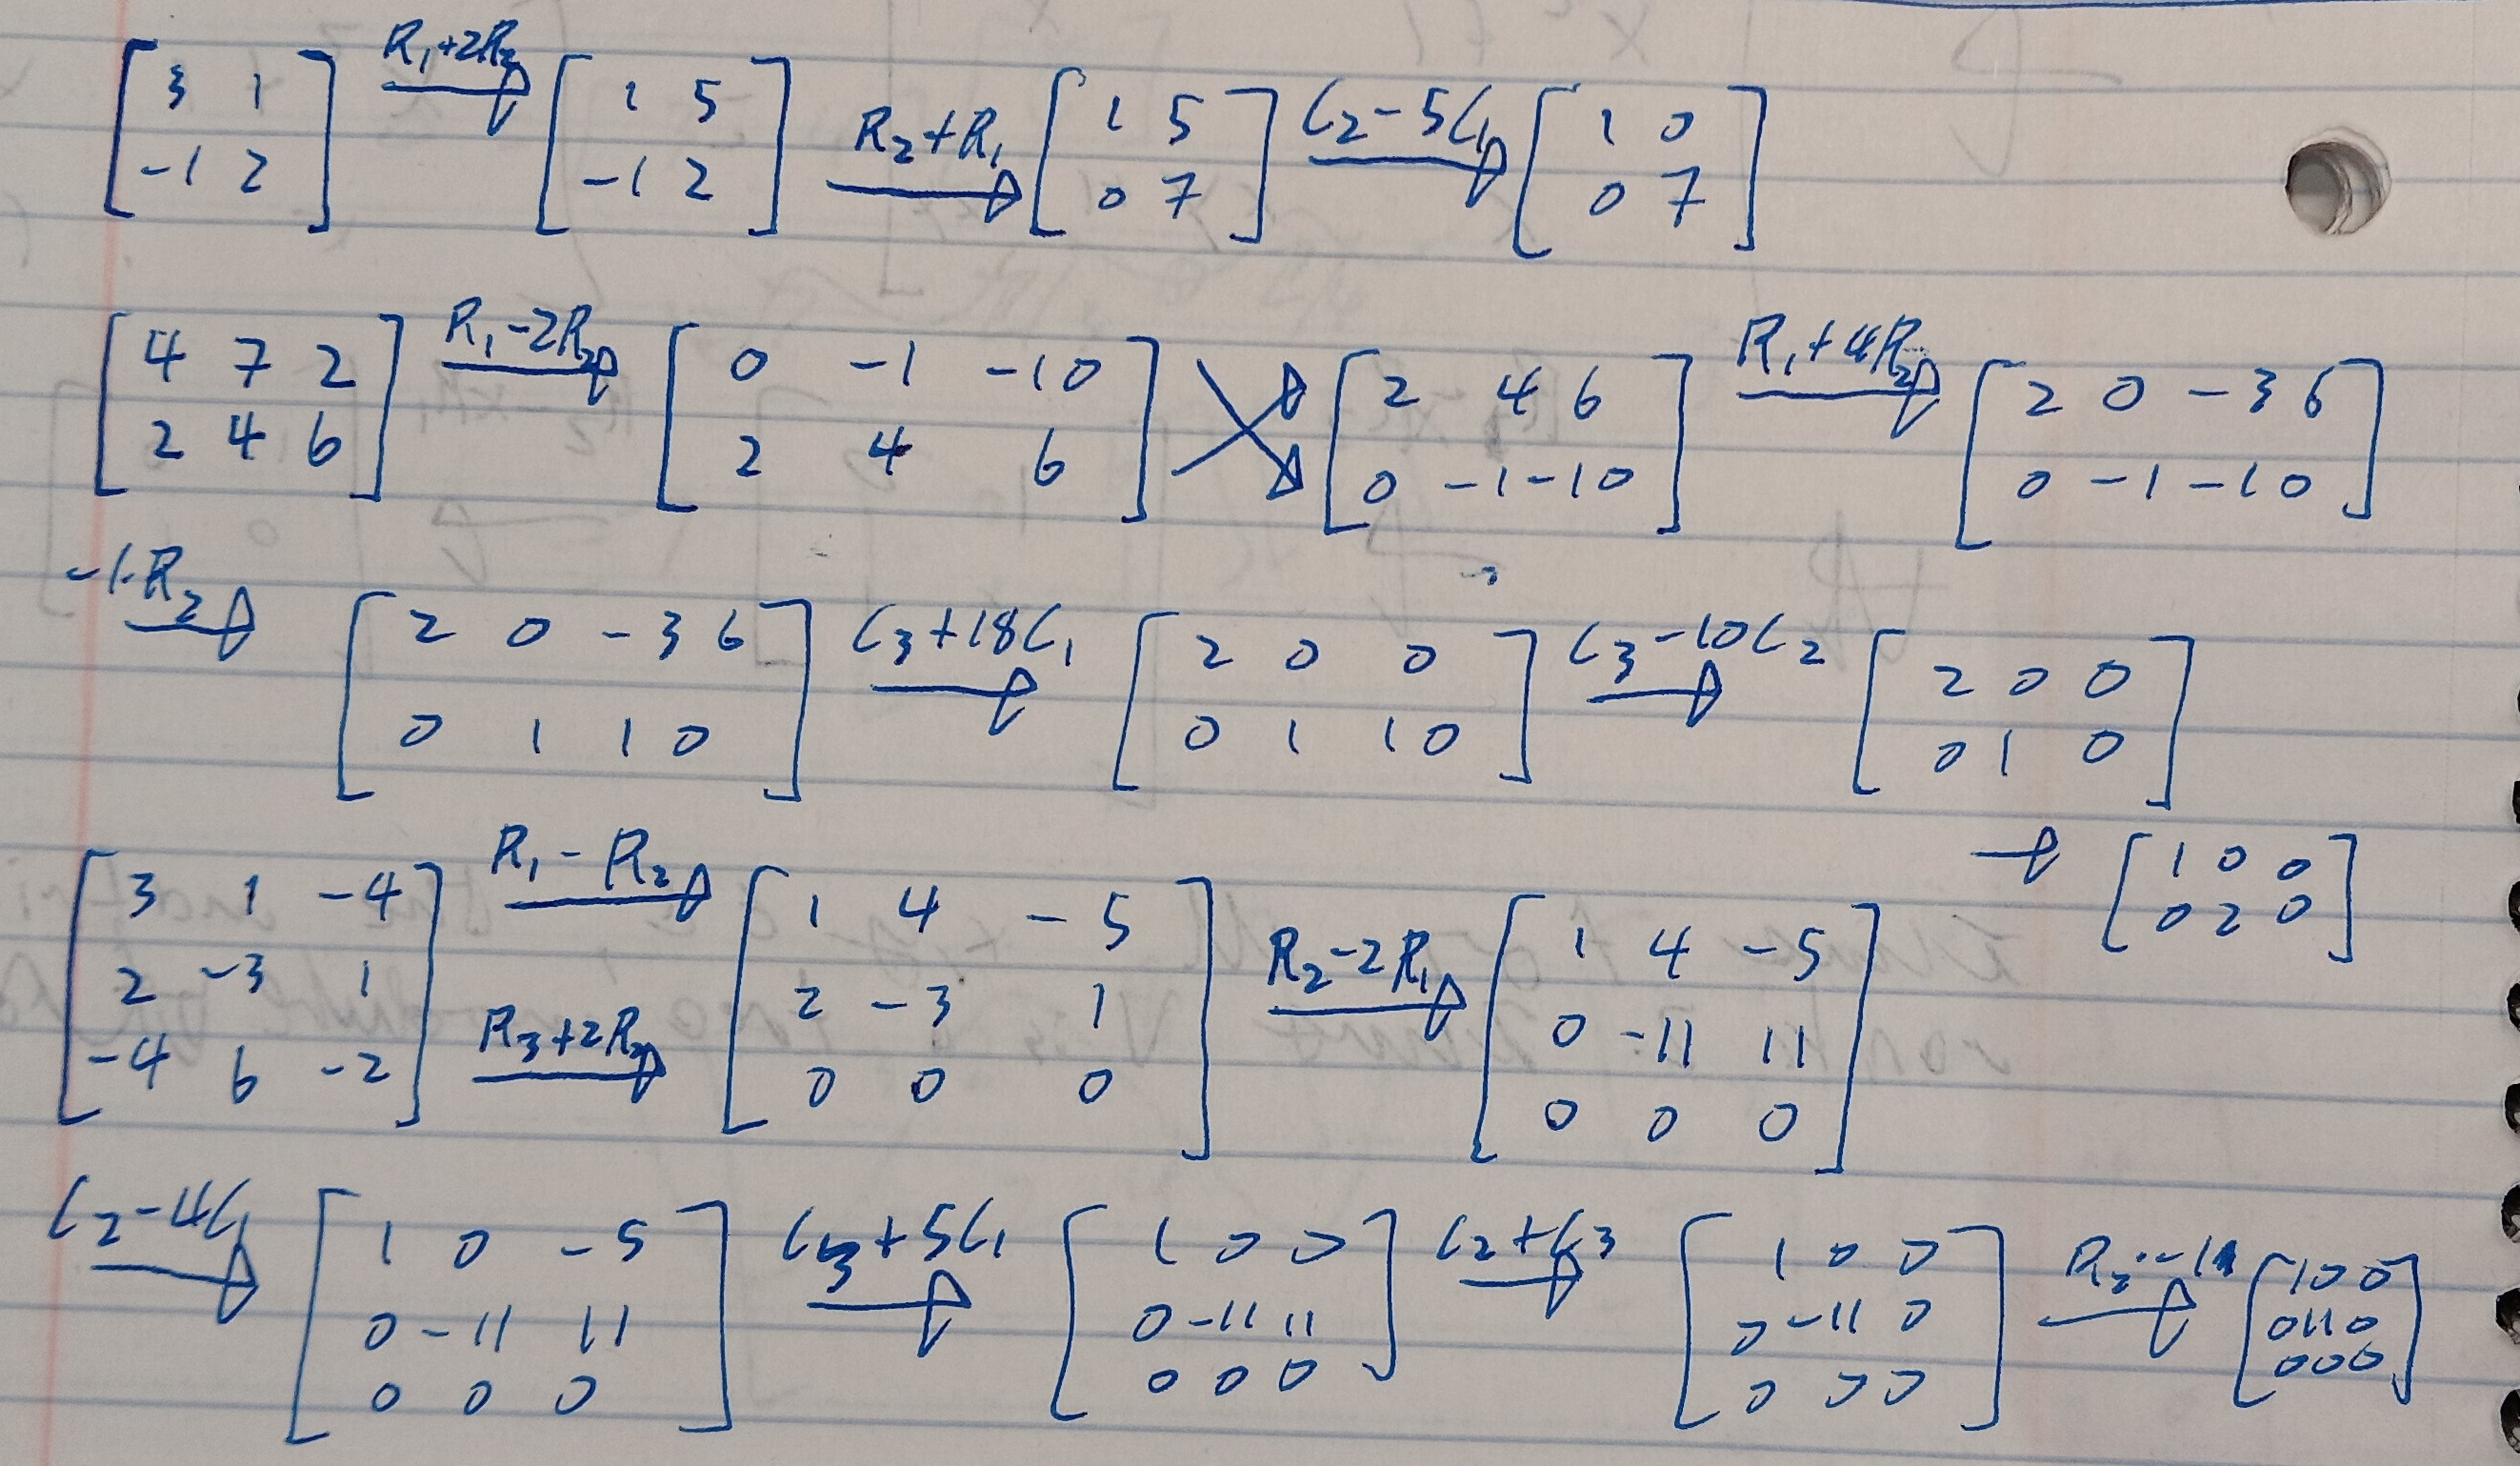
\includegraphics[scale=0.25]{20231206_154927.jpg}
	\item[4.6] 
	\begin{itemize}
		\item $\Rightarrow$ Suppose for contradiction that $A$ is singular.
		Then we know by problem 2.3 that it has a rank which is less than $k$.  
		This gives us that in smith normal form there are guaranteed to be at 
		least one zero in the diagonal.  Let $A' = Q^{-1}A P$.  Suppose this zero
		is at index $i \in [k]$ then if we take the vector $v' = (0,0,\cdots,1,1,\cdots, 1)$ then this vector must be orthogonal to the image of $A'$.  Since $P,Q$ 
		are invertible matrices, then the orthogonality is preserved, thus 
		$Q^{-1}vA$ is orthogonal to the image of $A'$.  Thus we can add subtract arbitrarily from the set $im A$ by $v = Q^{-1}v'A$ then we have an infinite number  cosets of $im A$ in $\Z^k$
		\item $\Leftarrow$ Suppose $A$ is non-singular.  Then it has smith normal form equivalent to $\begin{bmatrix}
		d_1 & 0 & \cdots & 0\\
		0 & d_2 & \cdots &0\\
		\vdots & \vdots & \ddots & \vdots\\
		0 & \cdots &  0 & d_k 
		\end{bmatrix}$
		Therefore a vector $v$ is in the cokernel of $A$ if there exists 
		$v' \in \Z_{d_1}\cdots \Z_{d_k}$.  Note that there is $d_1 \cdots d_k$ possible types of vectors in the cokernel (unscaled).  Thus there are $\det A$ 
		possible unscaled vectors in the cokernel.  Thus there are a finite number 
		of cosets.  
	\end{itemize}
	\item[6.1] Note that by Hilbert's theorem $\C[x_1,\cdots,x_n]$ is a noetherian
	ring.  Let us construct an ascending chain of ideals.  Start with $(f_1)$.
	Clearly $(f_1) \subseteq (f_1,f_2)$.  Furthermore $(f_1,f_2) \subseteq (f_1,f_2,f_3)$.  By induction we have an ascending chain of polynomial ideals.  
	However, since $\C[x_1,\cdots,x_n]$ is Noetherian then there exists $k \in \N$
	where $(f_1,\cdots f_k) = (f_1,f_2,\cdots)$.  Thus $\C[x_1,\cdots,x_n]/(f_1,\cdots,f_k) = C[x_1,\cdots,x_n]/(f_1,f_2,\cdots)$.  Therefore by theorem 11.9.1
	gives us that the set of common zeros of the set of infinite polynomials 
	is represented by a finite number of polynomials.
	\item[7.1]
	The matrix can be put into smith normal form as $\begin{bmatrix}
	2 & 0 & 0\\ 0 & 2 & 0\\ 0 & 0 & 2\end{bmatrix}	 $.  We know that smith 
	normal form corresponds bijectively with an abelian group.  Since there are no
	zeros in the diagonal, then the abelian group is simply $(\Z_2)^3$.
	\item[7.2] The abelian group is $C_\infty \oplus C_1$
	\item[9.1a] We can reduce the matrix $\begin{bmatrix} x^2+1 & x\\ x^2y + x + y & xy + 1 \end{bmatrix}	 $ to the identity matrix without division.  Therefore 
	the matrix has rank 2 for every $x,y \in \C$.  Thus the module presented by 
	this matrix is free.  
		
\end{enumerate}
\end{document}
